%-------------------------------------------------
%	Version: 0.0
%	fecha de entrega
%
%-------------------------------------------------

\documentclass[11pt]{report}

%packages
\usepackage{graphicx}
\usepackage{subcaption}

\usepackage[utf8]{inputenc}
\usepackage[spanish, es-nodecimaldot]{babel}
\usepackage{setspace}
\usepackage{ragged2e}

\usepackage{amsmath}
\usepackage{amsthm}
\usepackage{amssymb}
\usepackage{mathtools}
\usepackage{siunitx}

%path donde se encuentran las imagenes
\graphicspath{ {./figuras/} }

%---------------------------------------------------------------
%ABREVIACIONES DE COMANDOS

\theoremstyle{plain}
\newtheorem{thm}{Teorema}[chapter] % reset theorem numbering for each chapter

\theoremstyle{definition}
\newtheorem{defn}[thm]{Definición} % definition numbers are dependent on theorem numbers
\newtheorem{exmp}[thm]{Ejemplo} % same for example numbers

\newcommand{\chaptercontent}{
\section{Basics}
\begin{defn}Here is a new definition.\end{defn}
\begin{thm}Here is a new theorem.\end{thm}
\begin{thm}Here is a new theorem.\end{thm}
\begin{exmp}Here is a good example.\end{exmp}
\subsection{Some tips}
\begin{defn}Here is a new definition.\end{defn}
\section{Advanced stuff}
\begin{defn}Here is a new definition.\end{defn}
\subsection{Warnings}
\begin{defn}Here is a new definition.\end{defn}
}

\usepackage{biblatex}
%\addbibresource{Tarea1.bib}

\begin{document}

\begin{titlepage}
\title{Bitacora}

%-------------------------------------------------
%PORTADA
%-------------------------------------------------

	\centering
	{\scshape\LARGE Universidad Autónoma de Yucatán  \\ Facultad de ingeniería\par}
	\vspace{1cm}
	{\scshape\Large Kundalini yoga para el aprendizaje\par}
	\vspace{1.5cm}
	{\huge\bfseries Cuarentena de práctica\par}
	\vspace{0.7cm}
	{\begin{figure}[!h]
	\centering
    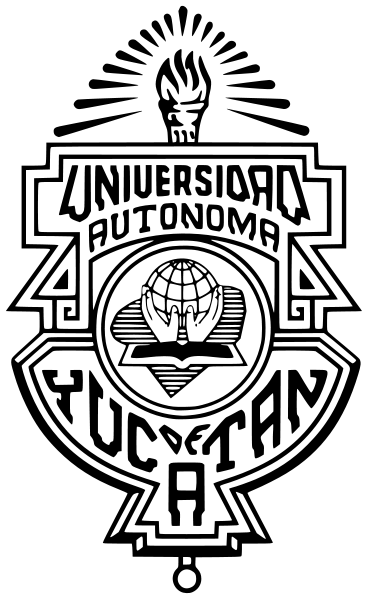
\includegraphics[scale=0.3]{UADY.png}
	\end{figure}}
	\vspace{0.7cm}
	{\Large\itshape Erick Al. Casanova Cortés\par}
	{\Large\itshape Matricula: 15014866\par}
	\vfill
	{\scshape\Large Docente\par
	Dra. María Milagrosa Pérez\par}
	\vfill
	{\Large{\bfseries Fecha de entrega: 7 Febrero 2021} }

	\vfill
	
\end{titlepage}

%-------------------------------------------------
%Inicio del documento
%-------------------------------------------------

\tableofcontents


\section{Introducción}

En el presente documento se relatará a manera de diario el transcurso de la cuarentena en práctica diaria de kundalini yoga. En este caso se eligió tanto un kriyas y una meditación para llevar a cabo durante la práctica. El kriya que se eligió fue el \textit{Sat kriya}, por el hecho de que estaba la facilidad de seguirlo desde YouTube; por parte de la meditación se optó por una serie de meditaciones como se verá a lo largo del trayecto, las cuales tienen el nombre de \textit{Vipassana} y \textit{Anapanasati}, ya que estas dos son meditaciones que ya había llevado desde hace tiempo y realmente me resultan bastante gratificante.\\
Como pequeña descripción de las meditaciones, ya que no fueron vistas en el curso, \textit{Anapanasati} consiste en sólo observar la respiración y ser consiente de la misma en todo el momento, mientras \textit{Vipassana} es la observación de las sensaciones haciendo un barrido por todo el cuerpo.

%-------------------------------------------------
%Bitácora
%-------------------------------------------------

\chapter{Bitácora}

\section*{Día 1}
	22/12/2020\\
	Hoy es mi primer día de práctica, terminé haciendo la práctica algo en la noche después de arreglar el cuarto y me sentí bastante bien, en sí la meditación se me hizo algo pesada pero logré hacer unos 20 minutos
	
\section*{Día 2}
	23/12/2020\\
	Este día preferí hacerlo antes de desayunar, en sí sentí que me ayudó bastante para despertar bien, seguí con \textit{Vipassana} como meditación pero aún siento que me distraigo mucho
\section*{Día 3}
	24/12/2020
	Hoy me levanté bastante tarde que no pude hacerlo en ayunas, y sentí bastante diferencia de hacerlo con algo dentro del estómago o no; creo que sí preferiré seguir haciéndolo al despertar
\section*{Día 4}
	25/12/2020
	Hoy se me paso darme tiempo para practicar
\section*{Día 5}
	Hoy sí me levanté temprano y pude realizar a gusto la práctica, siento que en si la meditación es lo que mas me esta costando trabajo, por lo que intentare otro tipo de meditación llamado \textit{Anapanasati} a partir de mañana
\section*{Día 6}%27
	A diferencia de los demás días, decidí practicar en la noche, igual sentí bastante bien tanto como el kriya y la meditación, aun siento que me esta costando trabajo seguir el kriya mucho tiempo, creo que a lo mas puedo aguantar dos minutos
\section*{Día 7}
	28/12/2020
	He estado algo cansado hoy y preferí solo meditar, igual se me juntó porque decidí empezar a hacer algo de ejercicio y se me hizo muy pesado, creo que tengo que dividir mas mis tiempos para que no se junte tanto la actividad física
\section*{Día 8}
	Me dolía todo el cuerpo del ejercicio de ayer y si me tomé un descanso para estar más confortable
\section*{Día 9}
	Con el descanso que me tomé ayer sentí que pude aguantar más el kriya esta vez, sigo aguantando lo mismo, pero ya lo siento menos laborioso
\section*{Día 10} %31
	Ya llevo más de una semana, aunque he fallado dos días siento que me está haciendo menos cansado, ya hasta mi gato me espera para las prácticas y siento que sí es más una práctica que se deba realizar por las mañanas, aunque implique dormirme temprano
\section*{Día 11} %1 enero
	1/1/2021
	Sí logré despertarme temprano, en sí aun no he sentido gran cambios en mi cuerpo, pero sí he sentido que la meditación me ha estado ayudando a poder concentrarme más en el día, o a estar más enfocado en las actividades que estoy haciendo
\section*{Día 12}%2 lol, 
	Casi todas las meditaciones que llevaba hasta ahora eran de unos veinte minutos, no lo sentía tan pesado desde que inicié, pero me gustaría tomarme más tiempo para meditar. Ya que solía antes hacerlo por lo menos una hora seguida y quiero ver si puedo retomarlo
\section*{Día 13}
	%dia 3
	Logré aumentar algo de tiempo en la meditación como me lo propuse ayer, aunque sí siento que por lo menos hacer solo \textit{Anapanasati} me ayuda bastante para relajar mi mente
\section*{Día 14}	
	Hoy se terminaron las vacaciones y realmente no tuve tiempo para hacerlo antes de desayunar, y sí no lo sentí tan confortable como las otras veces, pero aún así sentí que estuvo bastante bien, aproveché que uno de mis profes canceló su clase para poder practicar lo más temprano posible
\section*{Día 15}
	Tampoco me dio tiempo para practicar antes, tuve que dejarlo hasta la noche porque tuve todas mis clases y también algunas tareas por hacer. De por sí los martes me toca encargarme de toda la casa y no tuve tanto tiempo libre
\section*{Día 16}
	Hoy fue un día bastante tranquilo y logré seguir la práctica antes de desayunar, ya creo que puedo lograr hacer tres minutos sin tanto problema o sentirme mareado
\section*{Día 17}
	Traté de despertarme más temprano de lo normal, pero si me costó bastante trabajo tanto mantener el ritmo como las respiraciones, seguía dormitando bastante, creo que cambiaré a hacer las prácticas antes de dormir
\section*{Día 18}
	Sentí que apenas pude hacerlo, practique antes de dormir, pero ya me dolía la cabeza y preferí dormirme más temprano para aprovechar que mañana no tengo clases y despertarme temprano
\section*{Día 19}%sabado
	Esta vez preparé un té antes de la práctica porque igual me andaba durmiendo y sentí que aunque no fuese el estómago completamente vacío, bastante bien la práctica 
\section*{Día 20}%enero 10
	Ya es la mitad de la cuarentena y he empezado a sentir los cambios, desde que ya no me cuesta trabajo levantarme temprano hasta que puedo realizar el kriya más tiempo de lo que empecé, igual me gustaría retomar la meditación con la que inicié
\section*{Día 21}
	Igual creo que empezaré a aumentar a unos 2 minutos el kriya a ver como me va, por lo menos ahora con minuto y medio no lo siento tan fatigante como cuando inicié, igual con la meditación, ya casi retomo mis tiempos de meditar una hora seguida, creo que intentaré la siguiente vez meditar 40 minutos de los cuales 20 no moverme para nada
\section*{Día 22}
	Se me hizo algo pesado, pero logré levantarme temprano para hacer el kriya antes de desayunar. En general lo sentí bien
\section*{Día 23}
	Me gustó mucho este día, en sí sentí como todo estuvo muy bonito y sentí el cuerpo superbien, sigo pensando que es una práctica que debe ser en la mañana
\section*{Día 24}
	Ya a más de tres semanas siento que sí tengo más energía y me siento más activo en general, solo que sí siento como poco a poco la escuela me está consumiendo mi energía física y mental
\section*{Día 25}
	Casi todos los viernes son los días más pesados que tengo en la universidad, y sí apenas tuve chance de practicar hoy, en general la práctica me fue bien, solo me sentí algo estresado por la cantidad de proyectos que nos empezaron a marcar
\section*{Día 26}%sab
	Hoy me levanté temprano y logré hasta hacer ejercicio y todo se sintió bastante bien
\section*{Día 27}%dom
	Me tomé el día en general para descansar, casi siempre termino empezando la semana algo agotado y he sentido un circulo viscoso por lo mismo
\section*{Día 28}
	Si me sirvió lo de descansar, porque desperté sin problemas y no me estaba durmiendo en la meditación, igual trataré de no dormirme muy tarde hoy para poder levantarme temprano mañana
\section*{Día 29}
	A pesar de que no logré levantarme temprano, estuvo bien porque logré practicar en la noche
\section*{Día 30}
	Hoy inicié bastante motivado, a veces sí siento como un boost de energía después de los kriyas, y hoy lo sentí bastante bien, me ayudó bastante a concentrarme
\section*{Día 31}
	También logré levanterme temprano, me gustaría levantarme aún más temprano de lo que recurrentemente hago, pero igual implica dormir más temprano y a veces sí siento que no me da tiempo para eso, en cuanto a la práctica, sentí algo tediosa la meditación pero el kriya estuvo bastante bien, no me está cansando ni nada
\section*{Día 32}
	Hoy no tuve tiempo para hacerlo, me levanté bastante tarde y terminé algo agotado por lo mismo de que fue un día pesado y ya ni tiempo de arreglar mis cosas tuve
\section*{Día 33}%sab
	Como todos los sábados, logré levantarme temprano para poder practicar, me gusta bastante más hacerlo desde temprano por el clima y como me ayuda a despertar
\section*{Día 34}
	Igual me levante temprano y pude practicar sin problemas, tengo ganas de aumentar el tiempo del criya, aunque no sé bien cuando sería algo recomendado
\section*{Día 35}
	Aumenté a nos 5 minutos, y también lo sentí bastante cómodo, aunque sí al final me andaba cansando, creo que sí puedo aguantar los 5 minutos, solo es cosa de que me lo pronponga desde el inicio
\section*{Día 36}
	Con respecto a la meditación de hoy, la senti bastante fluida, no estuvo nada pesada y me gustó bastante, igual sí logré aguantar los cinco minutos del kriya sin problemas, espero mantenerlo así
\section*{Día 37}
	Casi y no lograba practicar hoy, me salieron bastantes pendientes y sí no los terminé todos pero por lo menos tuve unos quince minutos libres para dedicarlos a la práctica
\section*{Día 38}
	Hoy igual se me hizo algo pesado porque estuve bastante cargado de tareas, pero logré terminarlas antes de tiempo y me di chance para meditar un rato
\section*{Día 39}
	Siento que mi cuerpo ya anda bastante bien con el kriya, tanto como las clases de los miércoles me están ayudando para hacer algo extra de lo que hago y me anda gustando eso
\section*{Día 40} %sab
	A pesar de que hoy fue el último día de la práctica en sí, me gustaría seguir hacéndolo, intentaré mantener el ritmo de hacerlo diario, aunque se me está complicando por los tiempos, ya que sí me toma todo como una hora u hora y media del día; y justo muchas materias de las que estoy llevando están marcando muchos proyectos, tal vez lo que más me cueste es seguir con el habito de levantarme temprano

\chapter{Pensamientos después de los cuarenta días}
	En general sentí bastante bien mi cuerpo durante el transcurso de los cuarenta días, creo que en sí disfrutaba más hacerlo los fines de semana que entre semana, casi lo sentía más como un deber más que algo que hiciera por gusto, tal vez por lo apurado que de vez en cuando llegaba a estar o por lo mismo de que este semestre tuve una carga bastante pesada y hacía que se me complicara los tiempos. Por otro lado creo que seguir esta rutina diario me ayudó para trabajar con mi recurrencia en lo referente a mi persona, ya que antes de esto casi no le prestaba atención a mi cuerpo, o me di cuenta en las meditaciones que luego salían cosas que pensé ya había trabajado y salieron al aire de nuevo\\

	En sí le recomendaría esta práctica a cualquier estudiante, aunque sí siento lo que me ayudó más fue la meditación, aunque sea solo el kriya hace bastante la diferencia al empezar el día
%-------------------------------------------------
%Final del documento
%-------------------------------------------------

\end{document}
